\section{Resultados}

\subsection{Simulaciones}
De acuerdo al diseño planteado, se registraron los tiempos promedios de la función tqli, que es la sección que ha sido paralelizada, y también del código para un análisis por MIPS. Veáse en la figura \ref{fig:seq_n30}, el comportamiento de las partículas en tiempo para las partículas vecinas de $n_0 = 30$. Cabe notar que el comportamiento en tiempo de cada partícula es oscilatoria a excepción de $n_0 = 30$. El movimiento de esta partícula es constante, pues debido a su excesiva masa con respecto a sus vecinos que impedia el movimiento inercial.

\begin{figure}[h]
	\centering
	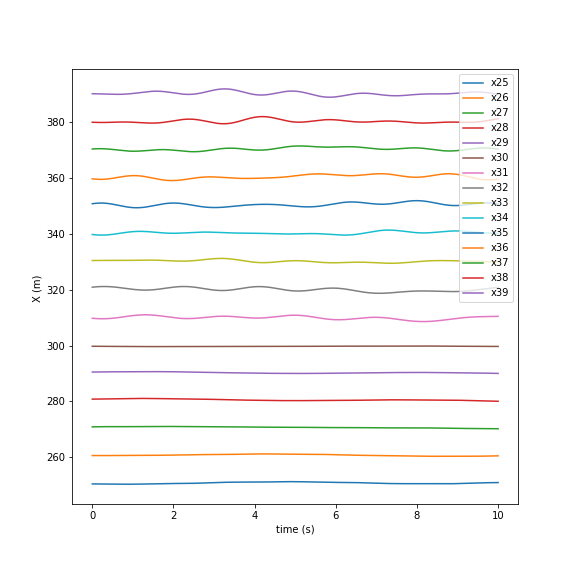
\includegraphics[width=0.4\textwidth]{seq_n30.png}
	\caption{Plot x25 a x40 en tiempo para n0 = 30} 
	\label{fig:seq_n30}
\end{figure}

En la figura \ref{fig:seq_n60_30}, se muestra el comportamiento para $n_0 = 60$ de las partículas entre 25 y 45. En ella se esalta que el comportamiento constante de la partícula $30$, yo no se presenta pues ahora $n_0 = 60$. Además, en la figura \ref{fig:seq_n60_60}, nuevamente se observe una de las lineas con comportamiento constante que representa el movimiento de la partícula $60$

\begin{figure}[h]
	\centering
	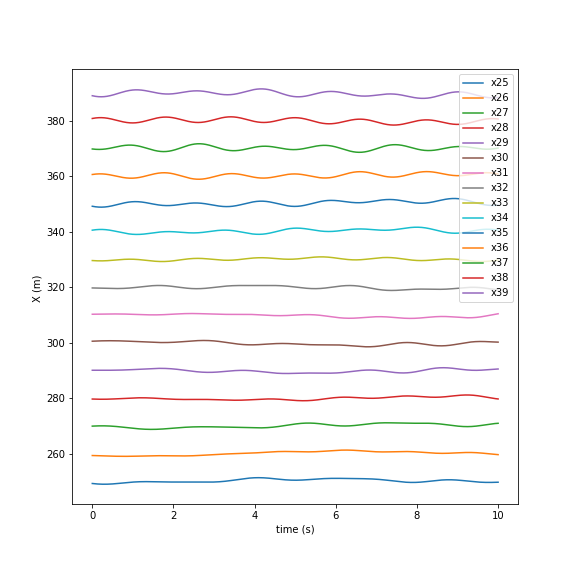
\includegraphics[width=0.4\textwidth]{seq_n60_30.png}
	\caption{Plot x25 a x40 en tiempo para n0 = 60}
	\label{fig:seq_n60_30}
\end{figure}

\begin{figure}[h]
	\centering
	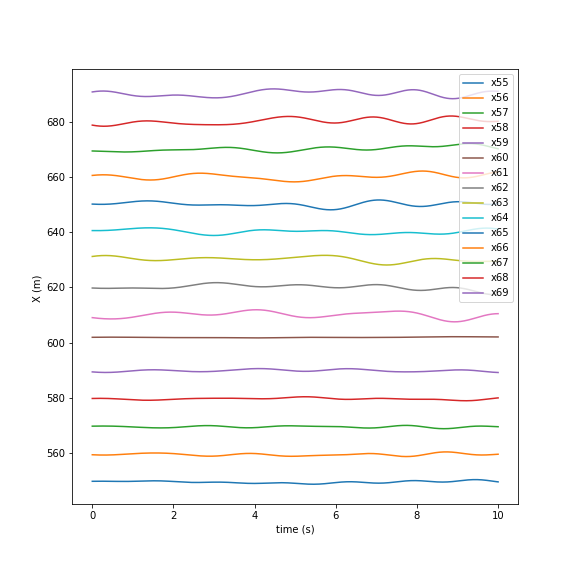
\includegraphics[width=0.4\textwidth]{seq_n60_60.png}
	\caption{Plot x55 a x70 en tiempo para n0 = 60}
	\label{fig:seq_n60_60}
\end{figure}

Cabe resaltar que convenientemente, se eligen los parámetros del sistema para que las oscilaciones sean correctas y aproximadamente reales.

\subsection{Desempeño en tiempo}
Para medir el desempeño, se corrieron los códigos múltiples veces hasta 10, y así obtener un valor promedio respecto a los procesadores.
En la figura \ref{fig:local_time_p}, se muestra el desempeño en tiempo. Notese que para distintos procesadores, el tiempo permanece siendo el mismo. Se justifica este comportamiento debido a que la sección paralela solo posee pocas operaciones y OpenMP implicitamente añade ciertos tiempos cuando se usa los statements pragma.

\begin{figure}
	\centering
	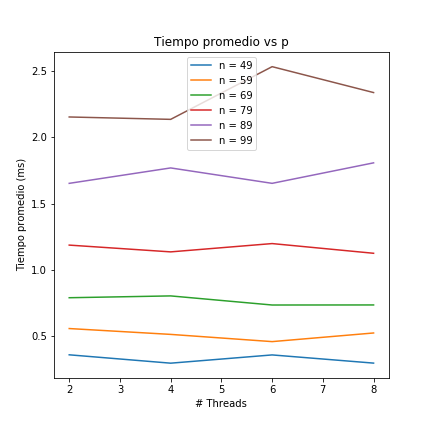
\includegraphics[width=0.35\textwidth]{local_time_p.png}
	\caption{Tiempo promedio de la función tqli respecto a numero de procesos localmente.}
	\label{fig:local_time_p}
\end{figure}
\begin{figure}
	\centering
	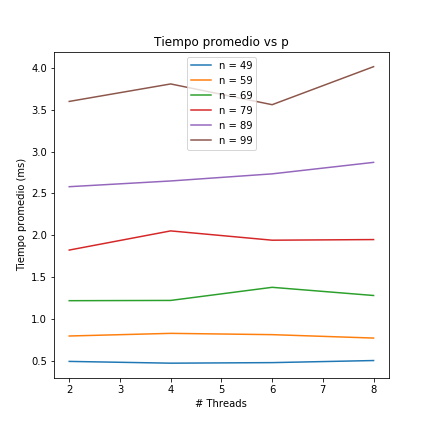
\includegraphics[width=0.35\textwidth]{server_time_p.png}
	\caption{Tiempo promedio de la función tqli respecto a numero de procesos en el servidor.}
	\label{fig:server_time_p}
\end{figure}


% b) Registrar el desarrollo de las simulaciones de manera ordenada en por lo menos 3 pasos (versiones beta)

% \subsection{Complejidad}

% Teorico:

% \begin{itemize}
% 	\item \textbf{Secuencial}:
% 	      hola
% 	\item \textbf{Paralelo}:
	      	          
% \end{itemize}

% Comparación con experimental, tiempo. Incluir graficos

\subsection{Velocidad}
Para medir la velocidad del programa, se decidió por usar la librería \text{perf} que puede calcular el número total de instrucciones y el tiempo de proceso. A partir de estos resultados se graficaron las figuras \ref{fig:local_time_p} y \ref{fig:server_time_p}. Notese que el comportamiento de todas las curvas no depende del numero de procesadores significativamente. Se puede justificar este comportamiento debido por la recursividad del algoritmo y la imposibilidad del paralelismos en todas sus secciones. Además, debido a su independencia del número de procesos, y la creciente respecto al número de elementos, también se dirá que el sistema no es escalable pues no cumple con la definición de convergencia de las curvas de velocidad.

%Medir velocidad del algoritmo en FLOPs. graficos

%Medir la escalabilidad del software

%e) Optimizar el software con un desarrollo orientado al paralelismo, y presentarlo
%en las conclusiones del paper


\begin{figure}
	\centering
	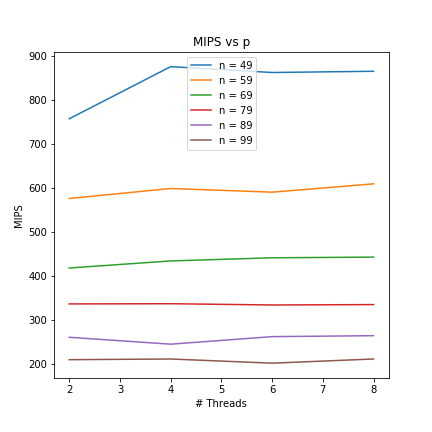
\includegraphics[width=0.35\textwidth]{local_mips_p.png}
	\caption{MIPS del programa respecto a numero de procesos localmente.}
	\label{fig:local_mips_p}
\end{figure}



\begin{figure}
	\centering
	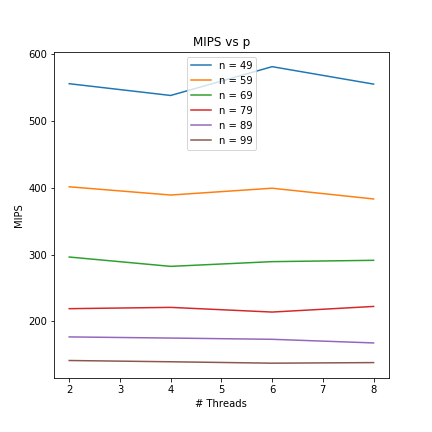
\includegraphics[width=0.35\textwidth]{server_mips_p.png}
	\caption{MIPS del programa respecto a numero de procesos en el servidor.}
	\label{fig:server_mips_p}
\end{figure}